% A line and the unit circle in the affine plane.
% Source: book/tex/riemann-surface/affine-projective.tex (§ Affine varieties).
\documentclass[border=2mm]{standalone}
\usepackage{tikz}
\usepackage{amssymb}
\usetikzlibrary{arrows.meta}
\begin{document}
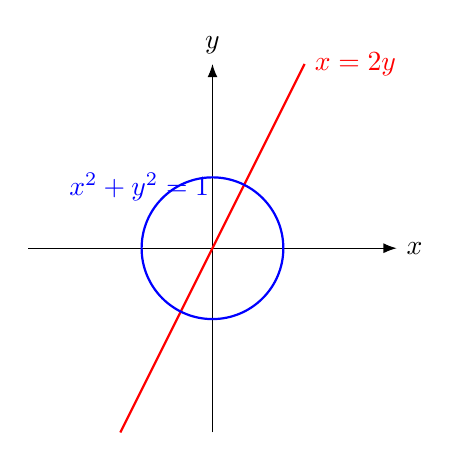
\begin{tikzpicture}[>=Latex,scale=0.9]
\draw[->](-2.6,0)--(2.6,0)node[right]{$x$};\draw[->](0,-2.6)--(0,2.6)node[above]{$y$};
\draw[red,thick](-1.3,-2.6)--(1.3,2.6)node[right]{$x=2y$};
\draw[blue,thick](0,0)circle(1);\node[blue] at(140:1.35){$x^2+y^2=1$};
\end{tikzpicture}
\end{document}
